%% Author: Chang Liu
%  Description: This template is used for generating the page head and foot
%  2015-03-27 00:15:10

\documentclass{article}
\usepackage{listings}	% add code segment
\usepackage{titlesec}   %set the page head/foot
%\usepackage{lastpage} % maybe used using Lastpages
%\usepackage{mathtools}
\usepackage{amsmath} % add math blod, boldmath, unbold
%\usepackage{graphics}
\usepackage{graphicx}
%\usepackage{picture}
%\usepackage{commath} % NOTE: use this with \abs to print the absolute value of E!!!
\usepackage[page]{totalcount}

\title{Algorithm Homework 5}
\author{Chang Liu}

\begin{document}

\newpagestyle{main}{            
    \sethead{Chang Liu}{HW5}{chang\_liu\\@student.uml.edu} % I don't know why here must use two "\" before to input @
    % and also know that strange error is often caused by the special characters.
    % here the \thepage is very useful to add for page number in the right part
    % \setfoot{}{}{\thepage} % just output the page number
    \setfoot{}{}{\thepage\ \// \totalpages} % add totalpages then needs page package and totalcount
    \headrule
    \footrule
}
\pagestyle{main}

\section{Two Kid Problem(15 points)}
\textbf{Question}: Professor Adam has two children who, unfortunately, dislike each other. The problem is so severe that not only do they refuse to walk to school together, but in fact each one refuses to walk on any block that the other child has stepped on that day. The children have no problem with their paths crossing at a corner. Fortunately both the professor’s house and the school are on corners, but beyond that he is not sure if it is going to be possible to send both of his children to the same school. The professor has a map of his town. Show how to formulate the problem of determining whether both his children can go to the same school as a maximum-flow problem.\newline


\textbf{Solution}: This problem could be thought of as a max flow problem.

1) Let the home be the source node and the school be the destination node.

2) For all other corners or crossing which could be visited by both of the children, we could assume a label $c_{i}$
to note these corners.

3) For every two corners, set a value $f(c_{i}, c_{j}) = 1$ if there is path that can be reached from $c_{i}$ to $c_{j}$, other nodes who connected to the corners or nodes interconnected have a weight that is more than 1, which could guarantee the minimum weight is one for each edge.

4) Then the problem could be described that: from the source to the destination, we assume the from one point to another
as a DAG(directed acyclic graph), if there exist a maximum flow which value is 2, then we could judge that there exist a
non-contradict path which could make both of the two children attend the same school.\newline


\textbf{Proof or Validness:}

We could know that apart from all other edges which weight is more than 1, if there is exist a solution that makes the
two children go to the same school, then they should either share some corners(because they can visit the corner, otherwise the home or school doesn't meet the requirement), or they just go in two different straight direction which
doesn\'st share any nodes.

For the first situation, since there are two children and they both visit this shared corner, so the incoming weight is
2, even though other nodes weight may be larger than 2, it is still 2 for these graph. We can know that other paths have
the weight equal or larger than 2, if smaller, then there must be negative weight.

For the second situation, we know that for two totally unrelated path, they share the source and ending point, their weight is 2 for maximum flow, other nodes that lay in the middle must have larger weights or at least, if two children we should combine it as $ 1 + 1 = 2 $, so max is still 2. 

So combining these two facts it's obvious that the max flow is 2 to solve the problem.

\section{Vertex Capacities(15 points)}
\textbf{Question}: Suppose that, in addition to edge capacities, a flow network has \textbf{vertex capacities}. That is each vertex $v$ has a limit $l(v)$ on how much flow can pass though $v$. Show how to transform a flow network $G=(V, E)$ with vertex capacities into an equivalent flow network $G^{'} = (V^{'},  E^{'})$ without vertex capacities, such that a maximum flow in $G^{'}$ has the same value as a maximum flow in $G$. How many vertices and edges does $G^{'}$ have?\newline

\textbf{Solution}: The original max flow problem with \textsl{vertex capacity} constrain could be converted to a non-vertex-capacity problem by the following changes:

1) for each vertex $v$, divide it into two separate vertex $v_{in}$ and $v_{out}$.

2) if there is an original edge $(u, v)$ in the old graph $G$, in our new graph $G^{'}$, we just need to make an
edge $(u, v_{in})$.

3) if there is an original edge $(v, w)$ in the old graph $G$, in our new graph $G^{'}$, we just need to make an
edge $(v_{out}, w)$.

4) for the two vertex $v_{in}, v_{out}$, we just need to make an edge between them and assign the capacity of this
edge to be the vertex capacity of original vertex $v$.

5) after all these rules setting, we could know that each new vertex $v_{in}, v_{out}$ don't have any vertex 
capacity constrains, the original constrain is shown by the edges of the two new vertex. But the overall max
flow is not changed as the incoming and outgoing edge capacity is not changed, so the network flow is not changed,
the vertex capacity constrain is added by the new edge comparing with old graph, but it is still the same constrain
condition as before, so the new solution is the same as the old one.

At last, we could know that in the new graph $G^{'}$, the added vertex is $|V|$, for the source vertex and end vertex,
we still need to divide them even though they don't have the incoming or outgoing flow, otherwise the vertex capacity
is not shown. For the edge we need to add $|E|$ to the original graph $G$. So in the new graph $G^{'}$, the edges are \boldmath\underline{$|V|+|E|$}\unboldmath, the vertex are \boldmath\underline{$2\times|V|$}\unboldmath.


\section{Modified Residual Network(15 points)}
\textbf{Question}: Suppose that we redefine the residual network to disallow edges into $s$. Argue that the procedure FORD-FULKERSON still correctly computes a maximum flow.\newline

\textbf{Solution}: Generally speaking, according to the FORD-FULKERSON method, when we want to calculate the maximum flow, we need to find the residual network and choose an augmenting path. Since this path's start point is $s$, so if we dismiss the edges into $s$, it still doesn't make any changes to the augmenting path, so the algorithm is the same as before's choice, and the final solution is still the same, since we would never choose the path that has the edge into the source $s$.


\section{$|E|$  Augmenting Paths(15 points)}
\textbf{Question}: Show how to find a maximum flow in a network $G = (V, E)$ by a sequence of at most $|E|$ augmenting paths. (Hint: Determine the paths after finding the maximum flow.)\newline

\textbf{Solution}: For this question, it's essential to record the maximum path for each iterations and then find the
ultimate one, which is the final maximum flow path. I would give a step by step description:

1) calculate the residual network for the original graph $G$.

2) then we could choose an augmenting path for this residual network generated above by using minimum cut, record this augmenting path so that it contains all the edges that forms a routine from source $s$ to sink $t$.

3) find the maximum weight or value for this augmenting path by using $min\{v_{1}, v_{2}, ... v_{n}\}$ in all the edges
for this augmenting path.($n$ is the size of this augmenting path)

4) apply this weight to the graph that generates the residual network, so that it will increase the flow for the edges
that in the augmenting path.

5) according to the new graph that has changed by step 4), regenerate the residual network like the step 1) shows.

6) do the operations from step 2) to step 5). If it can generate the residual network then keep looping, otherwise, If it cannot generate the residual network, then it has reached the maximum flow network, and the \textbf{last augmenting path} stored in step 2) is just the last changing path. We just need to check all the edges that go into the sink $t$, as ${t_{1}, t_{2}, t_{3}, ... t_{k}}$ shows, and the sum of them $\sum_{i=1}^k{t_i}$ is the maximum flow.($k$ is the size that counts to all the edges that go into the sink $t$), or select the edges that go out of the source $s$, as ${s_{1},s_{2}, s_{3}, ... s_{k\prime}}$ shows, and the sum of them $\sum_{i=1}^{k\prime}{s_i}$ is also the maximum(${k\prime}$ is the counts of edges that go out of the source $s$). Just like the below figure c) shows the source and sink nodes that the same as 11+12=19+4=23.

For the complexity of this algorithm, it is known that for each augmenting path, it will augment the graph G by one edge of the residual network, since each time it will select the minimum value of the path, and this will result in the maximum changes for this edge, and in the later rounds we will not select this edge since it reached its changing peak and cannot change anymore. So the extreme case is that each time we decrease one edge for the graph, and the overall cost is just the number of edges, which is $O(|E|)$;

\begin{center} % add this to make the figure shows in the middle of the pages
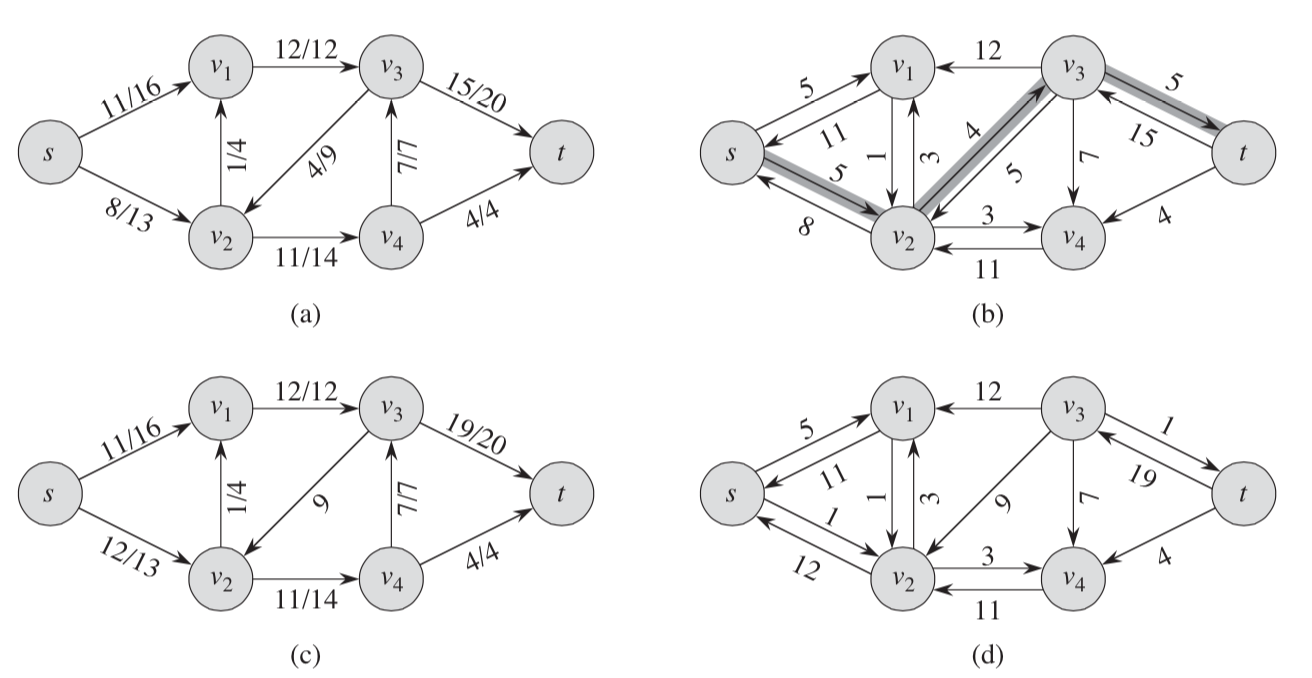
\includegraphics[width=4.00in,height=2.00in]{hw5_2.png}
\end{center}


\section{Max Flow by Scaling(20 points)}
\textbf{Maximum flow by scaling}

Let $G=(V, E)$ be a flow network with source $s$, sink $t$, and an integer capacity $c(u, v)$ on each edge $(u, v)\in{E}$. Let $C=max_{(u,v)\in{E}}c(u,v)$.

a. Argue that a minimum cut of $G$ has capacity at most $C|E|$.

b. For a given number K, show how to find an augmenting path of capacity at least K in $O(|E|)$ time, if such a path exists.

We can use the following modification of FORD-FULKERSON-METHOD to compute a maximum flow in $G$:

\begin{center} % add this to make the figure shows in the middle of the pages
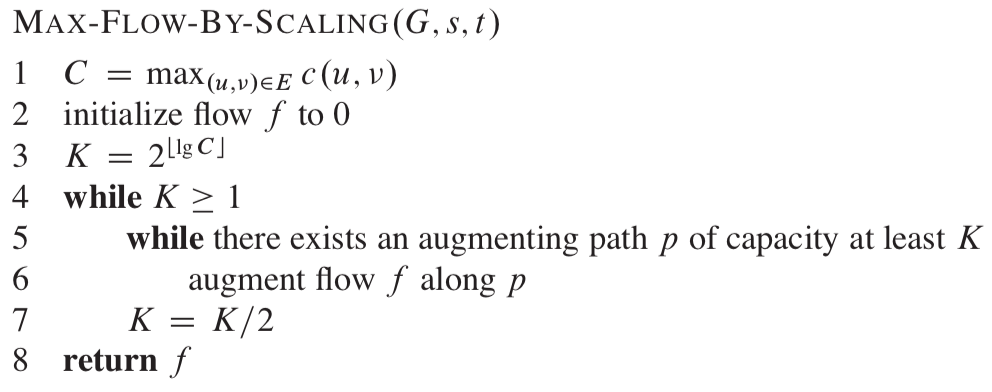
\includegraphics[width=4.00in,height=1.60in]{hw5_1.png}
%\caption{EHD descriptor for distinguishing the image}
\end{center}


c. Argue that MAX-FLOW-BY-SCALING returns a maximum flow.\newline

\textbf{Solution}:

a) For any cuts of the graph $G=(V, E)$, the capacity of one cut is as follows:
$$c(S, T) = \sum_{u\in{S}}\sum_{v\in{T}}c(u, v)$$

And a minimum cut is the cut which makes this capacity the least. We could know from the question that the maximum 
capacity of one edge is $C$, and the maximum edge that connects $S$ to $T$ is $|E|$, in this extreme graph, the capacity
of this cut reached the maximum capacity and its value is $C|E|$. And this extreme situation is also the maximum situation, so the minimum cut could be at most this value.

b) For this problem, when searching for an augmenting path, we could use the depth-first-search($DFS$) algorithm to start from the source $s$ to the sink $t$, while searching, if there are multiple choice, we should choose the minimum one that exceeds the value $K$, so that it will meet all the requirements that the capacity is at least $K$. The total cost for this algorithm is the $O(|V|+|E|)$ and in the flow network, the vertex is also treated as the function of $O(|E|)$, so that the overall cost is also the function of $O(|E|)$, so the complexity is $O(|E|)$.

c) First, we could know that $K=2^{\left \lfloor{\log{C}}\right \rfloor}$, where $C$ is the value of the maximum capacity of all the edges in the graph.

Second, for each iteration, it is known that the $K$ value is decreasing until it reaches the value 1, which is the power of zero, for each iteration it will decrease by linear, instead, the $K$ value could guarantee that the minimum
value is 1 so that the last iteration could solve the problem of some capacity that cannot augmented largely but need this small value 1 to adjust;

For decreasing process, since $K$  and $K/2$ value are all the capacity that lay in the graph, by scaling it is easy
to constrain the network flow and make it ends faster. But for this specific problem, according to \textbf{Theorem 26.6 (Max-flow min-cut theorem)}, it's shown that maximum flow is equal to no augmenting path in the residual network. According to the above description, after all the iterations it is guaranteed that it will end with no more augmenting path, so it is also the same conclusion which will return a maximum flow.


\end{document}